\documentclass{standalone}
\usepackage{tikz}
\usetikzlibrary{patterns, positioning}
\usepackage[sfdefault]{ClearSans} %% option 'sfdefault' activates Clear Sans as the default text font
\usepackage[T1]{fontenc}

\begin{document}
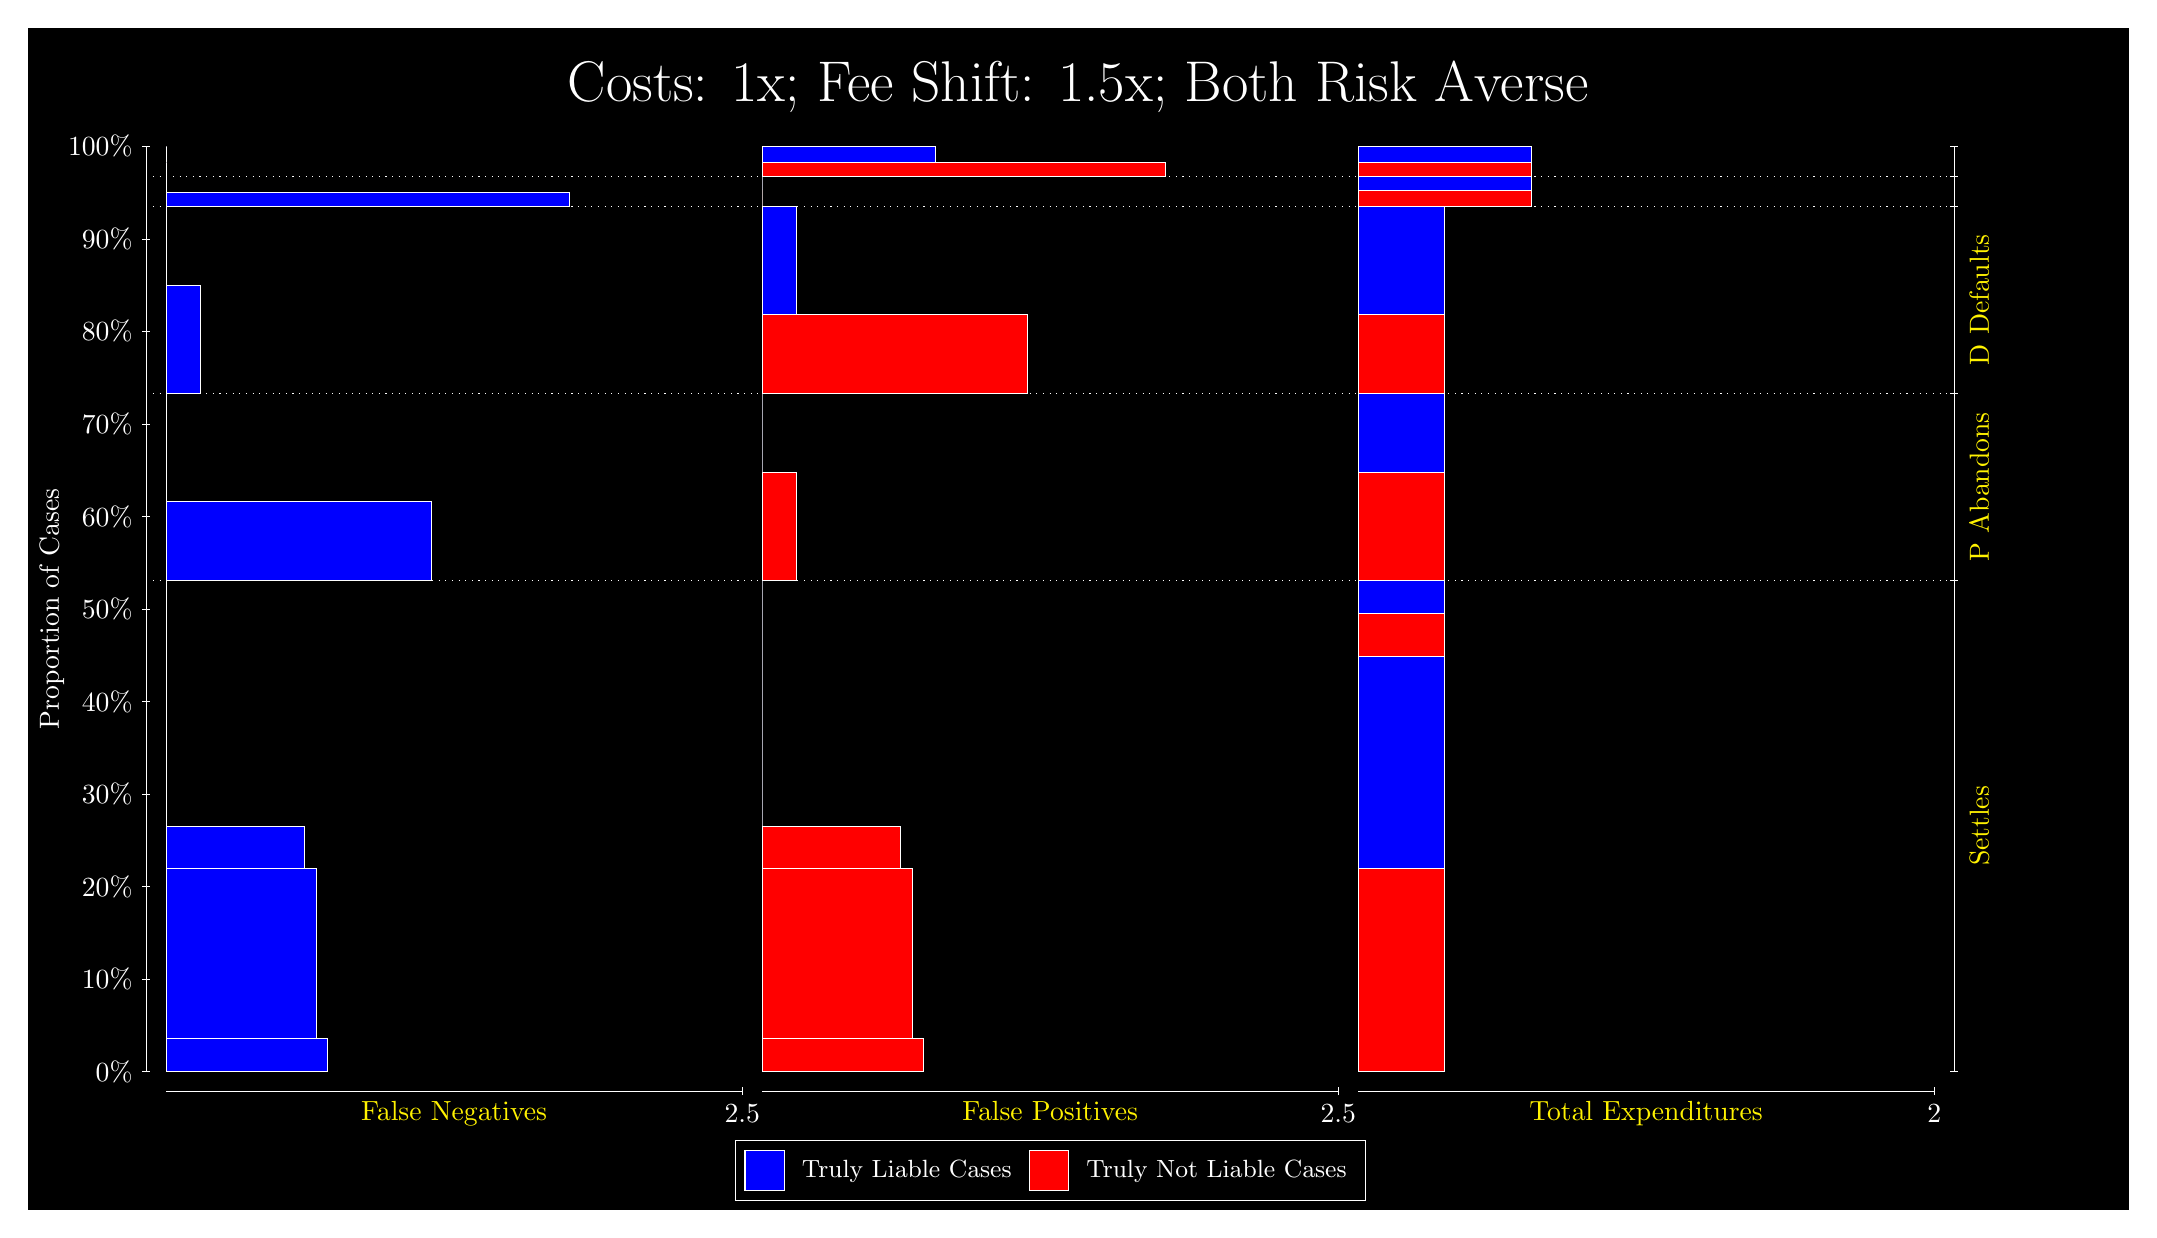
\begin{tikzpicture}
\draw[fill=black] (0,0) rectangle (26.667,15);
\draw[text=white] (0,13.5) rectangle (26.667,15) node[midway] {\huge Costs: 1x; Fee Shift: 1.5x; Both Risk Averse};
\draw[white, very thin] (1.5,1.75) -- (1.5,13.5);
\node[rotate=90, text=white, anchor=center] at (0.3, 7.625) {Proportion of Cases};
\draw[white, very thin] (1.45,1.75) -- (1.55,1.75);
\node[text=white, anchor=east] at (1.45, 1.75) {0\%};
\draw[white, very thin] (1.45,2.925) -- (1.55,2.925);
\node[text=white, anchor=east] at (1.45, 2.925) {10\%};
\draw[white, very thin] (1.45,4.1) -- (1.55,4.1);
\node[text=white, anchor=east] at (1.45, 4.1) {20\%};
\draw[white, very thin] (1.45,5.275) -- (1.55,5.275);
\node[text=white, anchor=east] at (1.45, 5.275) {30\%};
\draw[white, very thin] (1.45,6.45) -- (1.55,6.45);
\node[text=white, anchor=east] at (1.45, 6.45) {40\%};
\draw[white, very thin] (1.45,7.625) -- (1.55,7.625);
\node[text=white, anchor=east] at (1.45, 7.625) {50\%};
\draw[white, very thin] (1.45,8.8) -- (1.55,8.8);
\node[text=white, anchor=east] at (1.45, 8.8) {60\%};
\draw[white, very thin] (1.45,9.975) -- (1.55,9.975);
\node[text=white, anchor=east] at (1.45, 9.975) {70\%};
\draw[white, very thin] (1.45,11.15) -- (1.55,11.15);
\node[text=white, anchor=east] at (1.45, 11.15) {80\%};
\draw[white, very thin] (1.45,12.325) -- (1.55,12.325);
\node[text=white, anchor=east] at (1.45, 12.325) {90\%};
\draw[white, very thin] (1.45,13.5) -- (1.55,13.5);
\node[text=white, anchor=east] at (1.45, 13.5) {100\%};

\draw[white, very thin] (24.457,1.75) -- (24.457,13.5);
\draw[white, very thin] (24.407,1.75) -- (24.507,1.75);
\node[anchor=west] at (24.407, 1.75) {};
\draw[white, very thin] (24.407,7.9895) -- (24.507,7.9895);
\node[anchor=west] at (24.407, 7.9895) {};
\draw[white, very thin] (24.407,10.365) -- (24.507,10.365);
\node[anchor=west] at (24.407, 10.365) {};
\draw[white, very thin] (24.407,12.74) -- (24.507,12.74);
\node[anchor=west] at (24.407, 12.74) {};
\draw[white, very thin] (24.407,13.12) -- (24.507,13.12);
\node[anchor=west] at (24.407, 13.12) {};
\draw[white, very thin] (24.407,13.5) -- (24.507,13.5);
\node[anchor=west] at (24.407, 13.5) {};

\draw[white, very thin, fill=blue] (1.75,1.75) rectangle (3.7993,2.1716);
\draw[white, very thin, fill=blue] (1.75,2.1716) rectangle (3.6529,4.3283);
\draw[white, very thin, fill=blue] (1.75,4.3283) rectangle (3.5065,4.8697);
\draw[white, very thin, fill=red] (1.75,4.8697) rectangle (1.75,7.9895);
\draw[white, very thin, fill=blue] (1.75,7.9895) rectangle (5.1167,8.9906);
\draw[white, very thin, fill=red] (1.75,8.9906) rectangle (1.75,10.365);
\draw[white, very thin, fill=blue] (1.75,10.365) rectangle (2.1891,11.739);
\draw[white, very thin, fill=red] (1.75,11.739) rectangle (1.75,12.74);
\draw[white, very thin, fill=blue] (1.75,12.74) rectangle (6.8732,12.914);
\draw[white, very thin, fill=red] (1.75,12.914) rectangle (1.75,13.12);
\draw[white, very thin, fill=red] (1.75,13.12) rectangle (1.75,13.294);
\draw[white, very thin, fill=blue] (1.75,13.294) rectangle (1.75,13.5);
\draw[white, very thin, fill=red] (9.3189,1.75) rectangle (11.368,2.1716);
\draw[white, very thin, fill=red] (9.3189,2.1716) rectangle (11.222,4.3284);
\draw[white, very thin, fill=red] (9.3189,4.3284) rectangle (11.075,4.8698);
\draw[white, very thin, fill=blue] (9.3189,4.8698) rectangle (9.3189,7.9895);
\draw[white, very thin, fill=red] (9.3189,7.9895) rectangle (9.758,9.3636);
\draw[white, very thin, fill=blue] (9.3189,9.3636) rectangle (9.3189,10.365);
\draw[white, very thin, fill=red] (9.3189,10.365) rectangle (12.686,11.366);
\draw[white, very thin, fill=blue] (9.3189,11.366) rectangle (9.758,12.74);
\draw[white, very thin, fill=red] (9.3189,12.74) rectangle (9.3189,12.946);
\draw[white, very thin, fill=blue] (9.3189,12.946) rectangle (9.3189,13.12);
\draw[white, very thin, fill=red] (9.3189,13.12) rectangle (14.442,13.294);
\draw[white, very thin, fill=blue] (9.3189,13.294) rectangle (11.515,13.5);
\draw[white, very thin, fill=red] (16.888,1.75) rectangle (17.986,4.3284);
\draw[white, very thin, fill=blue] (16.888,4.3284) rectangle (17.986,7.0266);
\draw[white, very thin, fill=red] (16.888,7.0266) rectangle (17.986,7.568);
\draw[white, very thin, fill=blue] (16.888,7.568) rectangle (17.986,7.9895);
\draw[white, very thin, fill=red] (16.888,7.9895) rectangle (17.986,9.3636);
\draw[white, very thin, fill=blue] (16.888,9.3636) rectangle (17.986,10.365);
\draw[white, very thin, fill=red] (16.888,10.365) rectangle (17.986,11.366);
\draw[white, very thin, fill=blue] (16.888,11.366) rectangle (17.986,12.74);
\draw[white, very thin, fill=red] (16.888,12.74) rectangle (19.083,12.946);
\draw[white, very thin, fill=blue] (16.888,12.946) rectangle (19.083,13.12);
\draw[white, very thin, fill=red] (16.888,13.12) rectangle (19.083,13.294);
\draw[white, very thin, fill=blue] (16.888,13.294) rectangle (19.083,13.5);
\draw[white, dotted] (1.5,7.9895) -- (24.457,7.9895);
\draw[white, dotted] (1.5,10.365) -- (24.457,10.365);
\draw[white, dotted] (1.5,12.74) -- (24.457,12.74);
\draw[white, dotted] (1.5,13.12) -- (24.457,13.12);
\draw[white, very thin] (1.75,1.5) -- (9.0689,1.5);
\node[text=yellow, anchor=north] at (5.4094, 1.5) {False Negatives};
\draw[white, very thin] (9.0689,1.45) -- (9.0689,1.55);
\node[text=white, anchor=north] at (9.0689, 1.45) {2.5};

\draw[white, very thin] (9.3189,1.5) -- (16.638,1.5);
\node[text=yellow, anchor=north] at (12.978, 1.5) {False Positives};
\draw[white, very thin] (16.638,1.45) -- (16.638,1.55);
\node[text=white, anchor=north] at (16.638, 1.45) {2.5};

\draw[white, very thin] (16.888,1.5) -- (24.207,1.5);
\node[text=yellow, anchor=north] at (20.547, 1.5) {Total Expenditures};
\draw[white, very thin] (24.207,1.45) -- (24.207,1.55);
\node[text=white, anchor=north] at (24.207, 1.45) {2};

\node[text=yellow, centered, rotate=90] at (24.777, 4.8698) {Settles};
\node[text=yellow, centered, rotate=90] at (24.777, 9.1771) {P Abandons};
\node[text=yellow, centered, rotate=90] at (24.777, 11.552) {D Defaults};



\draw (12.978300999999998,1.5) node[draw=none] (baseCoordinate) {};
\begin{scope}[align=center]
        \matrix[scale=0.5, draw=white, below=0.5cm of baseCoordinate, nodes={draw}, column sep=0.1cm]{
            \node[rectangle, draw, minimum width=0.5cm, minimum height=0.5cm, fill=blue] {}; &
            \node[draw=none, font=\small, text=white] (B) {Truly Liable Cases}; &
            \node[rectangle, draw, minimum width=0.5cm, minimum height=0.5cm, fill=red] {}; &
            \node[draw=none, font=\small, text=white] (B) {Truly Not Liable Cases}; \\
            };
\end{scope}

\end{tikzpicture}
\end{document}